\documentclass[11pt, oneside]{article}   	% use "amsart" instead of "article" for AMSLaTeX format
\usepackage{geometry}                		% See geometry.pdf to learn the layout options. There are lots.
\geometry{letterpaper}                   		% ... or a4paper or a5paper or ... 
%\geometry{landscape}                		% Activate for rotated page geometry
%\usepackage[parfill]{parskip}    		% Activate to begin paragraphs with an empty line rather than an indent
\usepackage{graphicx}				% Use pdf, png, jpg, or eps§ with pdflatex; use eps in DVI mode
								% TeX will automatically convert eps --> pdf in pdflatex		
\usepackage{amssymb}
\usepackage[version=4]{mhchem}

%2SetFonts

%SetFonts


\title{Expanding the Modeling of Type Ia Supernovae}
\author{Abigail Bishop}
%\date{}							% Activate to display a given date or no date

\begin{document}
\maketitle

% Something about an Abstract here.

\section{Introduction}

  % What is a Supernovae, specifically Type Ia and define subchandra
  
  % Why is it important for astronomy and why should we simulate it
  
  % How are these things typically simulated
  
  Supernovae (SNe), the explosive deaths of stars, are some of the most spectacular events in the universe. A special kind of supernovae, the Type Ia Supernovae, is especially notable for its use as an astronomical measure of distance. Type Ia supernovae occur when two stars are in orbit around each other. At least one star has already died once and has become a white dwarf (WD) usually with a mass around that of our sun, called a solar mass ($M_{\odot}$). Material in the outer shells of the WD's partner can be stolen by the WD through its gravitational field. Once the WD has taken enough material to reach a mass of 1.4 times $M_{\odot}$, it explodes. This 1.4$M_{\odot}$ is called the Chandrasekhar mass. The explosion releases light of many colors and other wavelengths. The graph plotting how bright each wavelength of light is in the explosion is the spectrum. Since these stars usually have the same mass and elemental composition when they explode, the explosions have the same brightness and uniquely Type Ia SNe spectrum. 
  
  An observational astronomer can observe an event resembling a Type Ia SNe and use its spectrum to confirm it is a Type Ia Supernovae. The astronomer can then take the brightness of the explosion and use it to calculate how far away the supernovae is. By using Type Ia SNe in other galaxies to measure how far away they are and other measurements, observational cosmologists have been able to measure the rate at which our universe is expanding. Without accurate models of Type Ia SNe, these calculations would not be possible. 
  
  The dilemma is that not all Type Ia Supernovae wait until their mass reaches  the Chandrasekhar mass of 1.4$M_{\odot}$ before they explode. Some explode at lower masses, in the subChandra range where their mass is less than 1.4$M_{\odot}$. This means the overall brightness and the spectrum of the explosion is slightly different from the Chandrasekhar mass Type Ia Supernovae. If an observational astronomer uses a subChandra Type Ia supernovae to measure distance, they will calculate a larger distance if they assume it is a Chandrasekhar mass star. This means, as computational nuclear astrophysicists, we need to model subChandra Type Ia SNe to help the observational astronomers make accurate calculations of astronomical distance. This has been done before, however, a paper by Ken Shen and Lars Bildsten has pointed out that previous simulations have not included as many possible nuclear reactions as it should have to make the calculations accurate. In this thesis I discuss the methods by which we use a computer code to simulate Type Ia SNe with the elements suggested by Shen and Bildsten. 

\section{Codes}

  \subsection{GitHub}
  	
    GitHub is a website used to mediate code sharing and code collaboration. Most of the codes discussed in this report are available online, with all code available for viewing, editing, and using. This is the concept behind open-sourced software. 

  \subsection{Pynucastro}
    
    Pynucastro is an open-sourced coding package developed by Dr. Michael Zingale and Dr. Donald Willcox to create networks of nuclear reactions that can be used in their simulations. %Cite Pynucastro paper
    It does so by collecting information on the rate at which nuclear reactions occur at different temperatures from a database called AMREX. The formatted reaction rates are compiled into a network that can be access by simulations like Microphysics and Castro. 
  
  \subsection{Microphysics}
  
    Microphysics is an open-sourced software, available on the StarKiller GitHub repository, with routines designed to incorporate aforementioned networks of reaction rates into astrophysical simulations. % Cite Microphysics
    It is equipped with unit tests designed to run stellar simulations in a short amount of time to troubleshoot problems on a small scale before promoting the simulations to a larger scale operation. Microphysics comes with some preexisting networks but can also use new networks generated by Pynucastro. 
  
  \subsection{Castro}
  
    Castro is an open sourced software, available under the AMReX-Astro repository on GitHub, and is designed to run full scale simulations of astrophysical events in one dimension, two dimensions, and three dimensions. Simulations include Type Ia SNe, core collapse SNe, and WD mergers. 
  
\section{Motivation}
  
  As previously mentioned, Type Ia SNe are critical to measuring large astronomical distances. Observational astronomers rely heavily on accurate estimations for what they observe to make scientific claims to the data. In a 2016 paper by Lars Bildsten and Kenneth Shen, they theorized that the three elements used to simulate Type Ia supernovae was not enough to accurately simulate the spectra and light curve of a Type Ia supernovae. %Cite Shen and Bildsten
  Additionally, not all Type Ia SNe occur when the WD becomes a total of 1.4 $M_{\odot}$, sometimes the explosions set off, they detonate, before the Chandrasekhar mass is reached. This means that thesIt is critical that accurate models of Type Ia SNe are obtained in order for observational astronomers to learn about the universe accurately. 
  
  The goal for this research is to first create a nuclear reaction network following Shen and Bildsten's guidelines, test the network in Microphysics to see if there is a substantial change, then to run an old model and the new model with Castro using a sub-Chandrasekhar mass star to see how the results change. If the change is drastic, then we will have more science to do. 
  
\section{Simulation Results}

  \subsection{Pynucastro}
    
    {\tt Aprox13} is a nuclear reaction network composed of 13 element isotopes. It begins with Helium (\ce{^4He} also known as an $\alpha$ particle) adds two \ce{^4He} to get a Carbon (\ce{^{12}C}) and one photon ($\gamma$) then continues to add $\alpha$ particles until Iron (\ce{^{56}Fe}) and a lot more $\gamma$'s are obtained. Since each isotope is connected by an $\alpha$ particle, this is called an $\alpha$ chain and earns the name 13 from the 13 isotopes on the $\alpha$ chain that it possesses. All elements that are \ce{^{24}Mg} and heavier are also connected through a process where an $\alpha$ particle hits an isotope and creates a new particle but kicks out a proton, then a different proton hits the new nucleus and one of those $\alpha$ chain isotopes are created along with a $\gamma$. In total the {\tt aprox13} network contains 22 isotopes and has proven to be a good model of stellar evolution, but Shen \& Bildsten suggest developing the reaction network more for Type Ia SNe. %Cite the heck out of Frank Timmes
    
    The study began through the use of Pynucastro to create the {\tt subch} network, standing for sub-Chandrasekhar. The network is composed of 8 reactions, each as suggested by Shen \& Bildsten. %Cite Shen and Bildsten
    
    \begin{align}
            \ce{3 ^4He &->  ^{12}C + 2\gamma } \\ 
            \ce{^{12}C + ^4He &->  ^{16}O + \gamma } \\
            \ce{^{14}N + ^4He &->  ^{18}F + \gamma } \label{chemeq:1.1} \\
            \ce{^{18}F + ^4He &-> ^{21}Ne +  \text{p}} \label{chemeq:1.2} \\
            \ce{^{12}C + p+ &-> ^{13}N + \gamma } \label{chemeq:2.1} \\
            \ce{^{13}N + ^4He &-> ^{16}O + \text{p}} \label{chemeq:2.2} \\ 
            \ce{^{16}O + ^4He &-> ^{20}Ne + \gamma } \\
            \ce{^{14}C + ^4He &-> ^{18}O + \gamma } \label{chemeq:3.2}
    \end{align}
  
  \subsection{Microphysics}
  
    This new network is now used in Microphysics. There is a unit test in Microphysics referred to as {\tt burn\_cell} which is simulates the chemical evolution in one zone of a star. This test is first used to what tolerance will optimize results and reduce computation time in this simulation. Using these results, the {\tt burn\_cell} test will be used to simulate the chemical evolution of this zone as nuclear reactions take place to use and generate different elemental isotopes. 
  
    \subsection{Testing Simulation Equation Tolerances}
  
      Tolerances are parameters used to gauge how accurately the equation solvers in the simulation are doing their job. A smaller tolerance typically leads to a more precise answer but takes more computer time. For this reason, a tolerance of $10^{-12}$ was treated as an exact answer and the tolerances of $10^{-3}$, $10^{-6}$, and $10^{-9}$ were tested. 
      
      %Say what other initial conditions you needed like temperature and such. 
     
      To test these tolerances, a fraction of  \ce{^4He}, \ce{^{12}C}, and \ce{^{16}O} were initialized in one zone as modeled by the {\tt burn\_cell} unit test. The zone is heated so that the three elements begin to burn. Simulations are run with a tolerance of $10^{-3}$, $10^{-6}$, $10^{-9}$, and $10^{-12}$. The relative error in each element's mass fraction, $X$, between the 3 former simulations and the $10^{-12}$ simulation, as defined by 
    
      \begin{equation}
        \sigma_X = \frac{X_{10^{-12}} - X_{\text{former}}}{X_{10^{-12}}} \text{    , }
        \label{eq:relativeerror}
      \end{equation}
    
      for each point in time during the simulation. This relative error in mass fraction is plotted as a function of time for each of the three testing simulations and can be seen in Figure~\ref{fig:relativeerror}.
    
      \begin{figure}
        \centering
        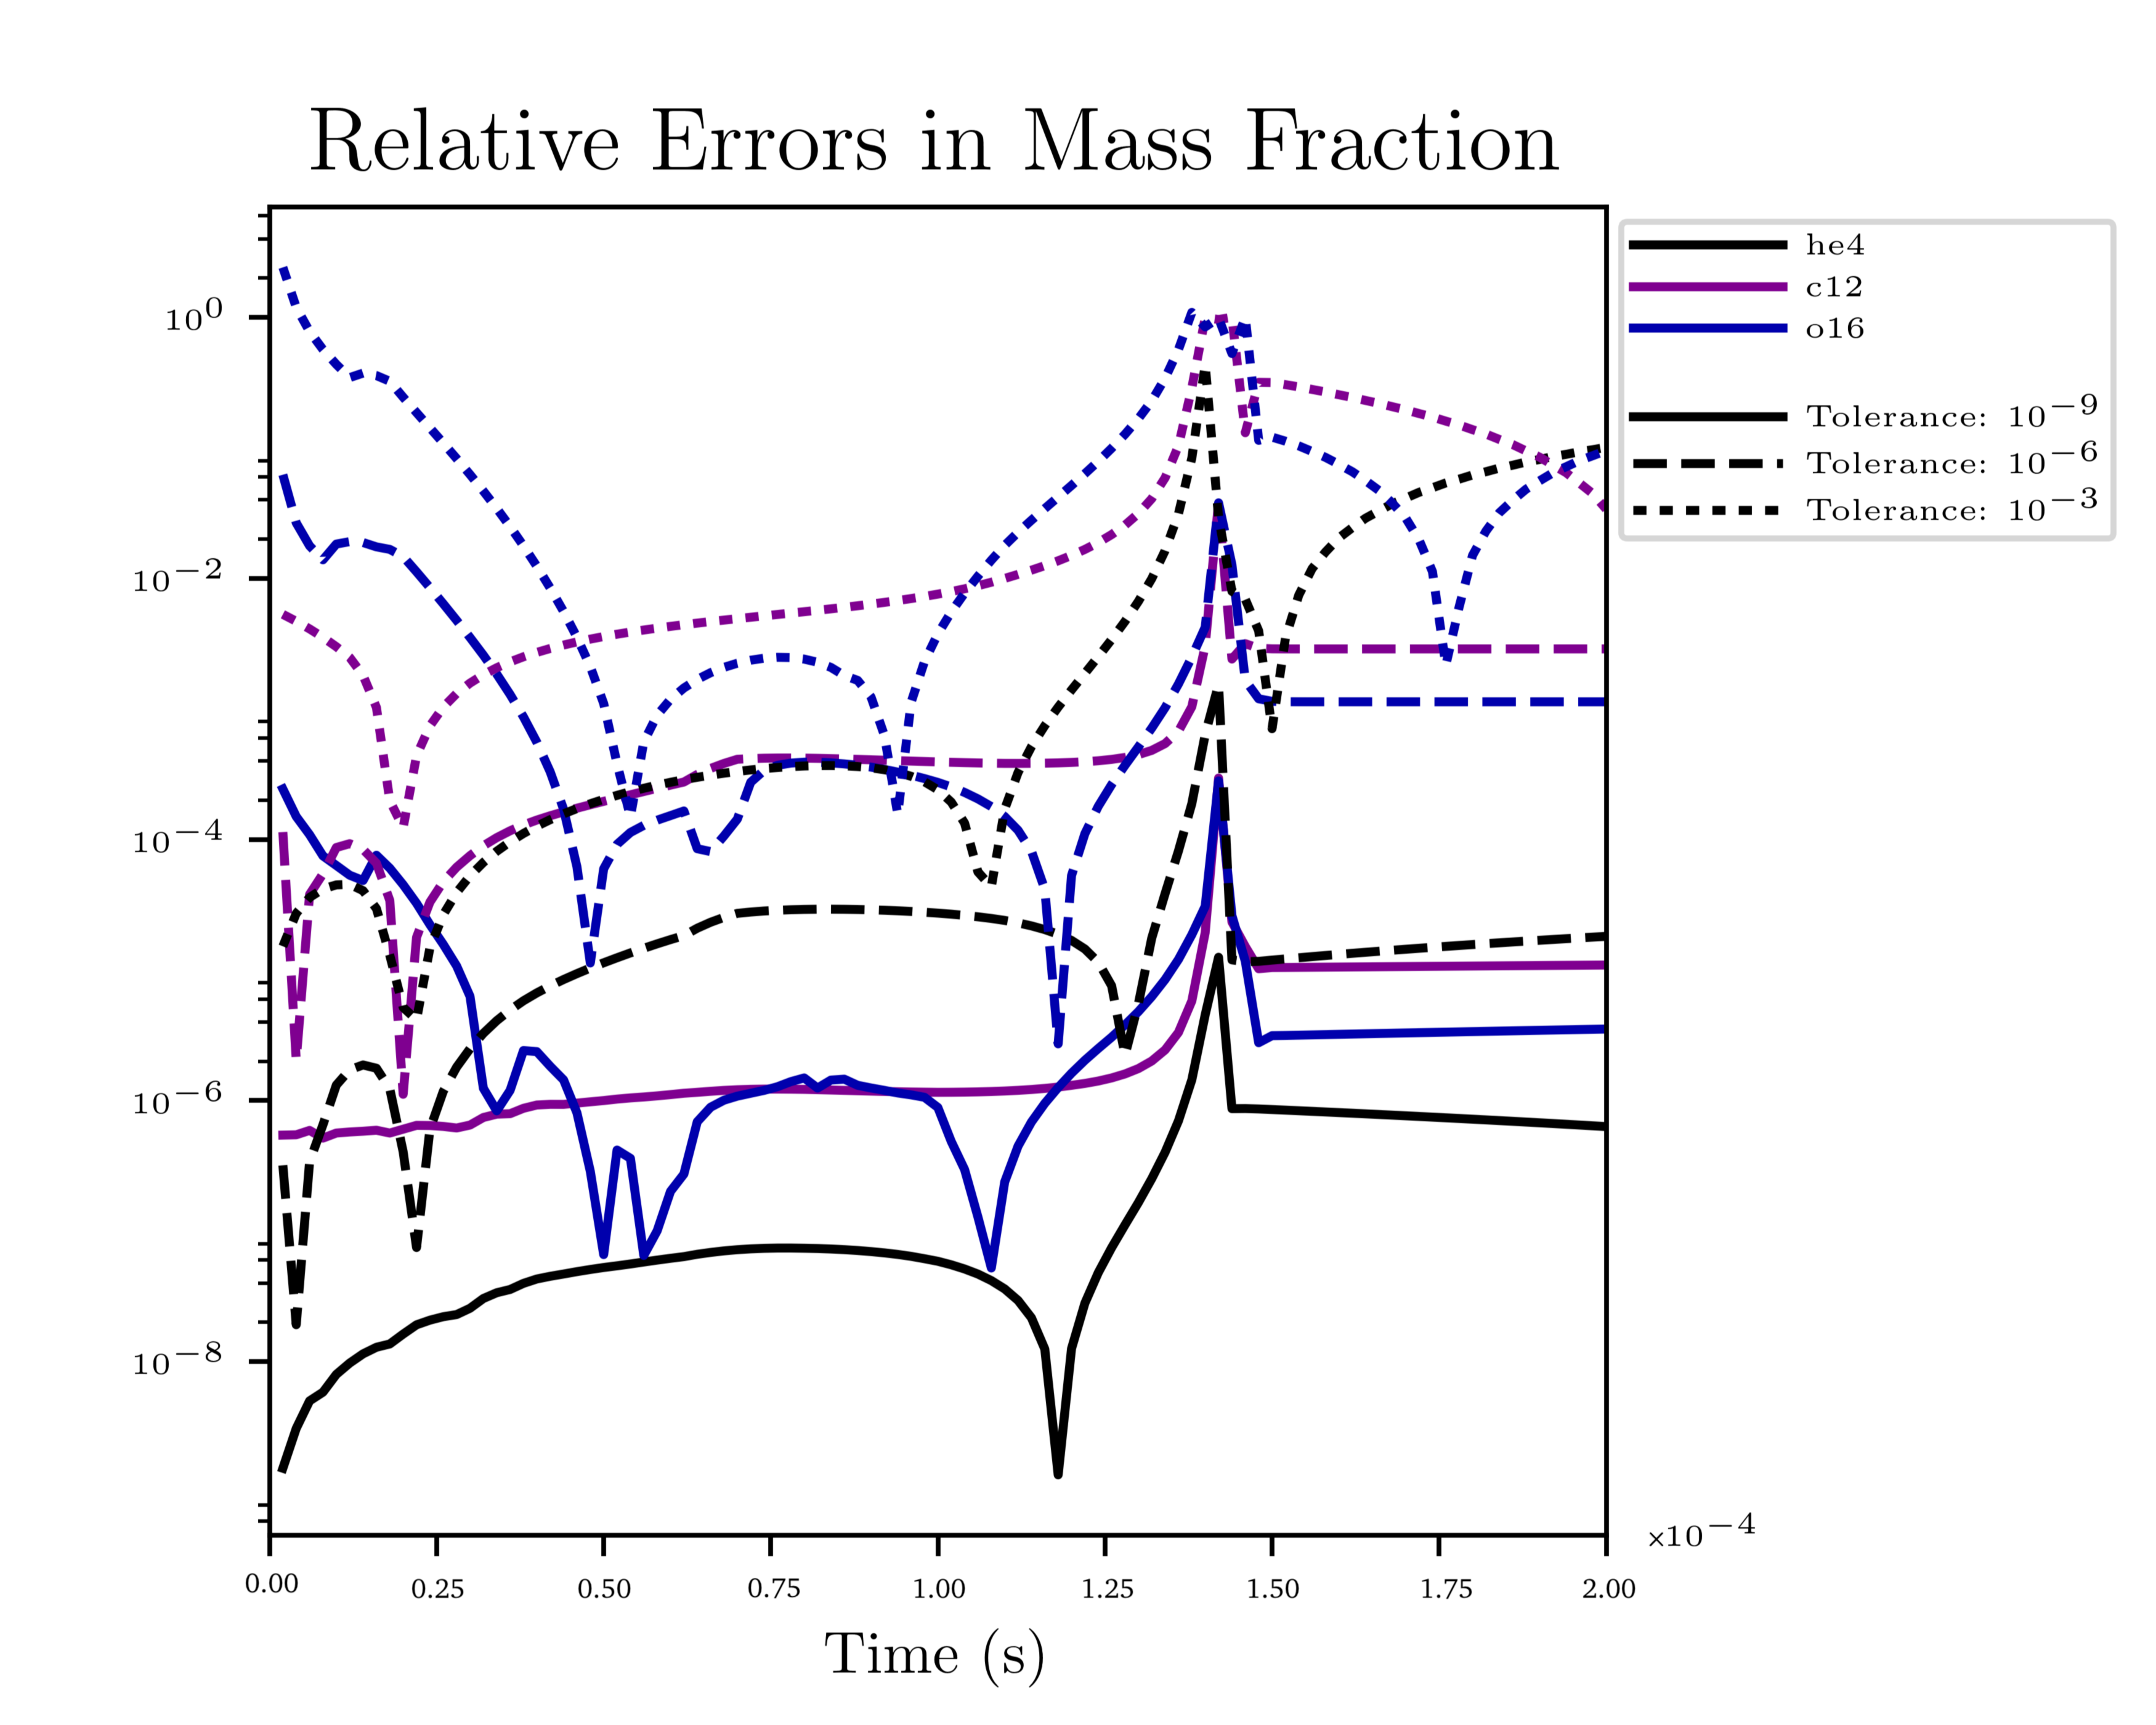
\includegraphics[width=5in]{images/react_aprox13_test13_ureca_tol-rel_xn1.png}
        \caption{}
        \label{fig:relativeerror}
      \end{figure}  
  
      From Figure~\ref{fig:relativeerror}, one can see that the solid lines, corresponding with the simulation using a tolerance of $10^{-9}$, are consistently the lowest. The corresponding run did not require very much run time and produced low-error results, therefore it is concluded that a tolerance of $10^{-9}$ is acceptable for the codes going forwards. 
  
    \subsection{Using Mass Fraction Evolution to Justify Motivation}
    
      The next step with the {\tt burn\_cell} tests is to test if the {\tt subch} network is producing results worth investigating. The main ingredients to the simulation that Shen \& Bildsten encouraged were \ce{^{14}C} and \ce{^{14}N}. % Cite Shen and Bildsten
      Figure~\ref{fig:microphysicsX} shows the time evolution of mass fractions, $X$, for each of the eleven isotopes in the {\tt subch} network for three different {\tt burn\_cell} simulations. The solid line corresponds to a simulation without \ce{^{14}C} and \ce{^{14}N}, the short dashed line adds some \ce{^{14}N} and the long dashed line adds both \ce{^{14}C} and \ce{^{14}N}. If this Shen \& Bildsten's theory is correct, we shouldn't see 11 clean and solid lines, but many more solid and dashed lines. Indeed, Figure~\ref{fig:microphysicsX} shows this and pushes us to take these simulations to the next level.
      
      %Say what other initial conditions you needed like temperature and such. 
      
      \begin{figure}
        \centering
        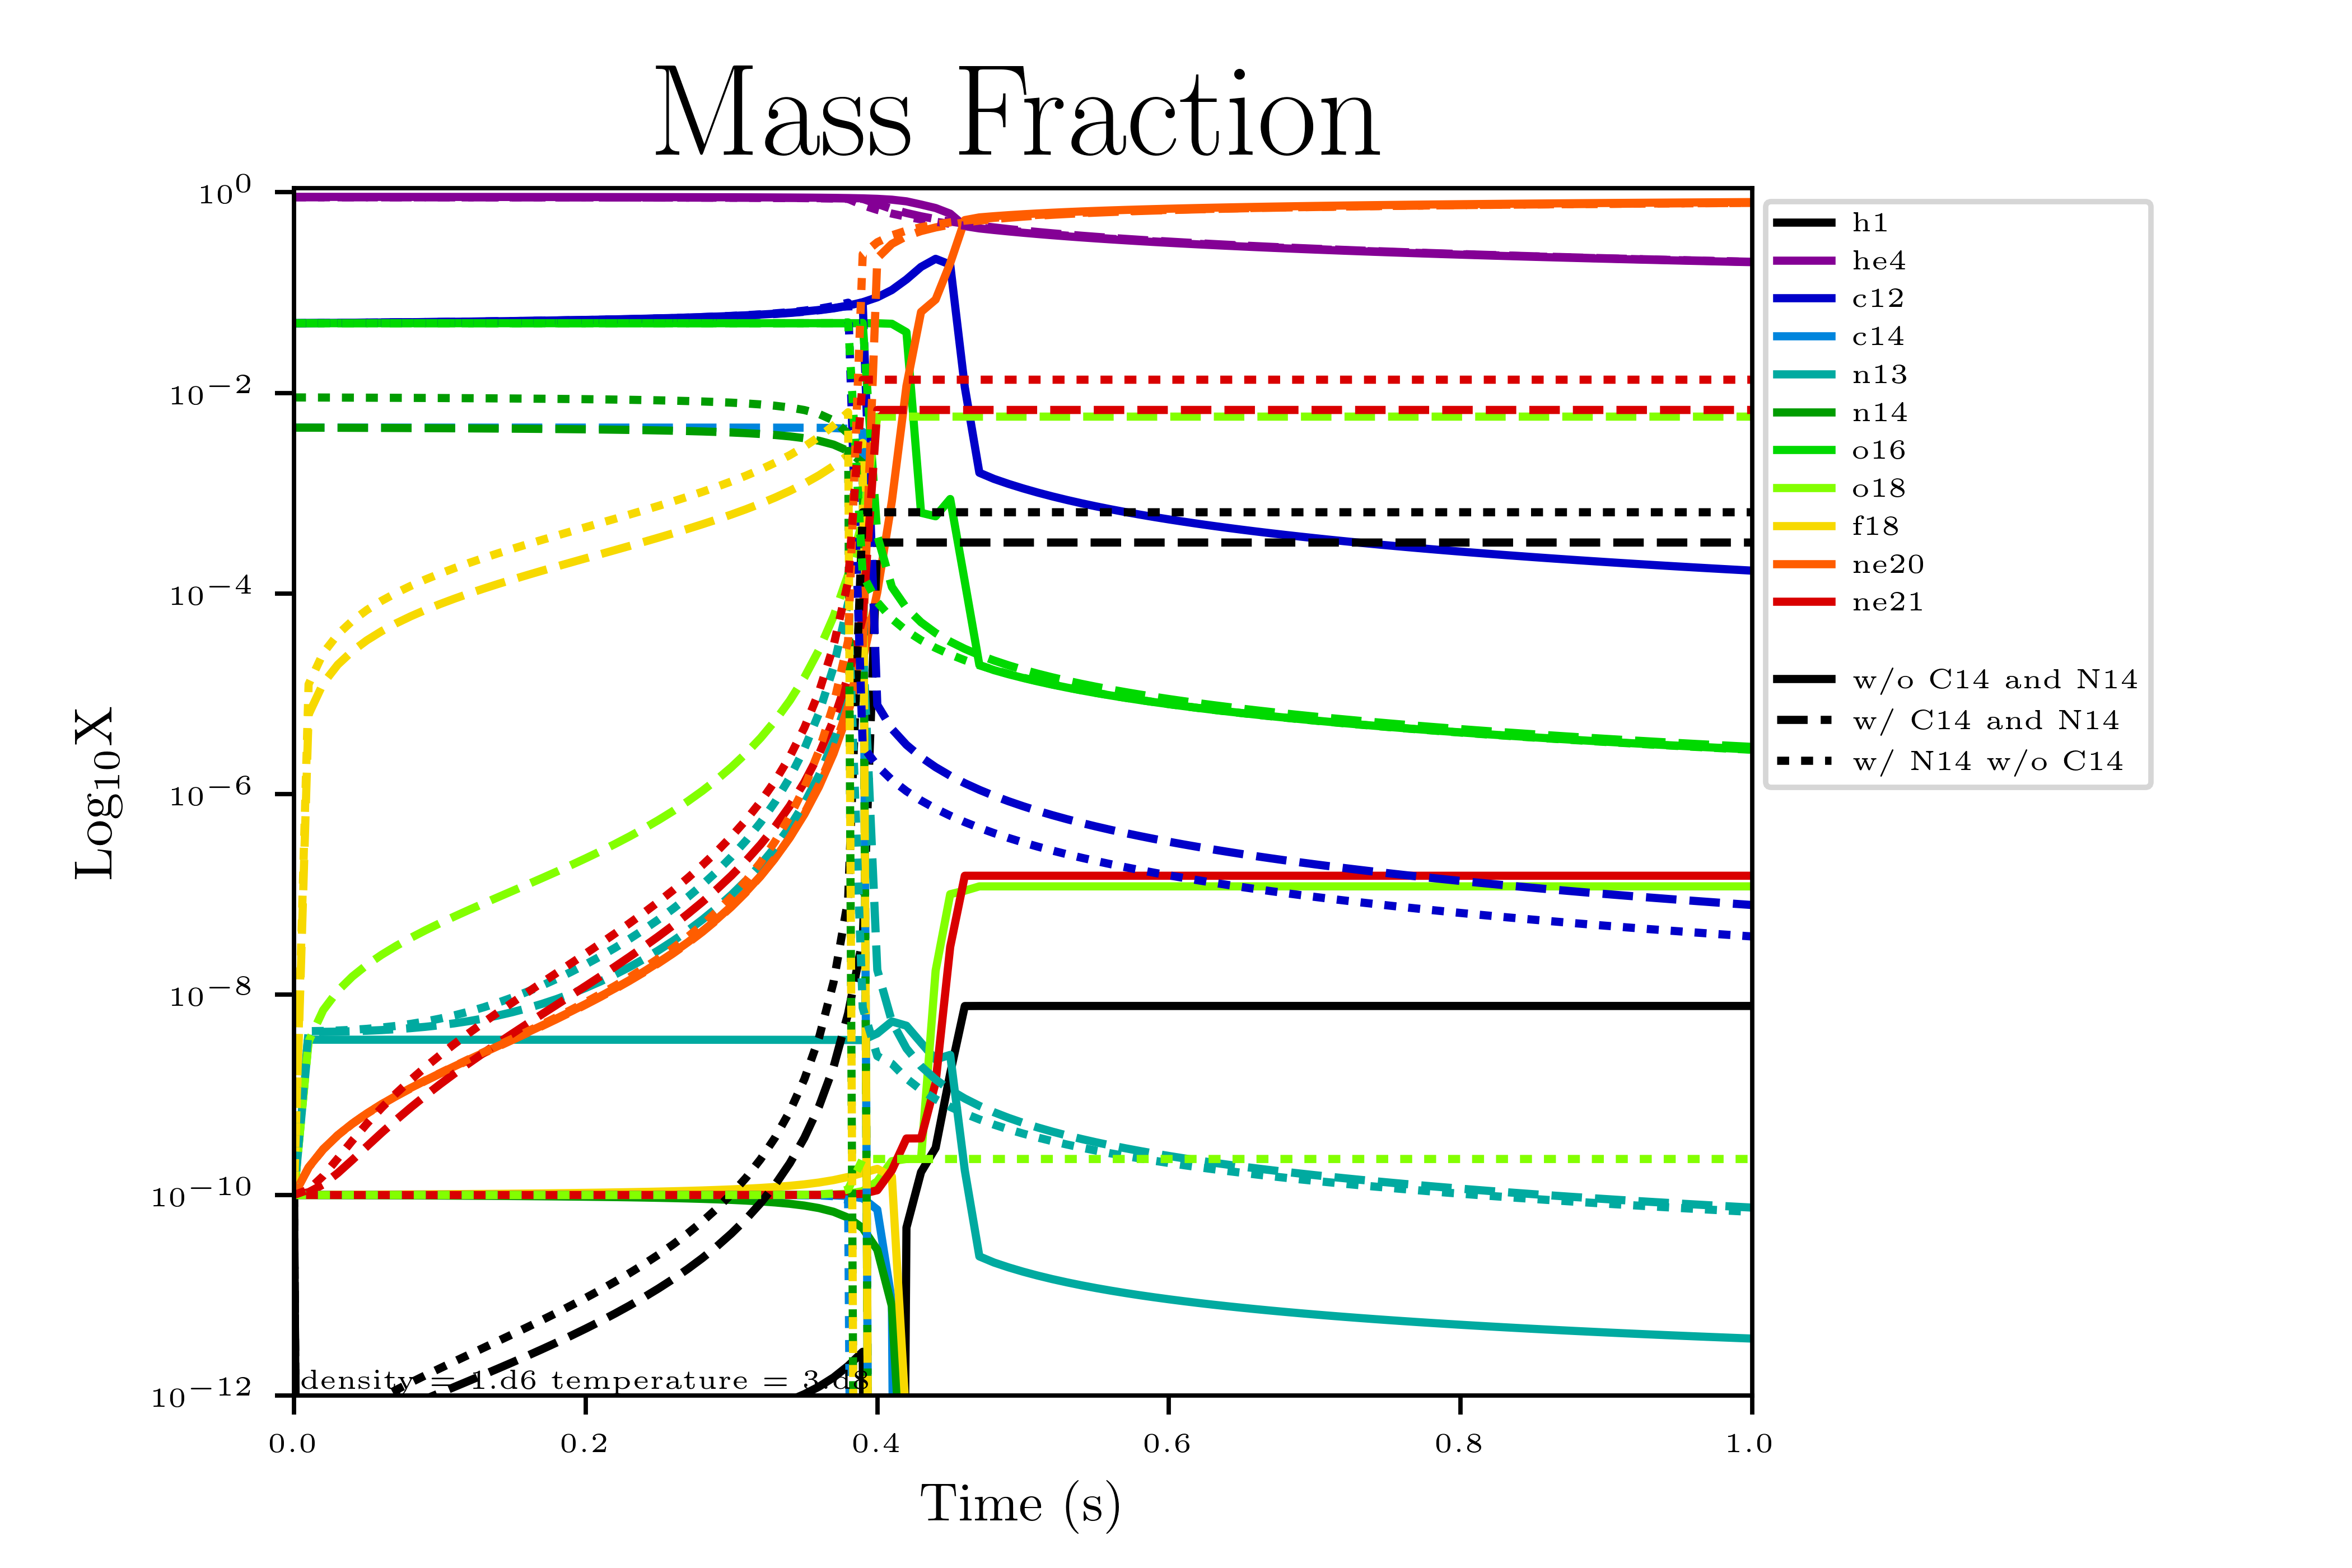
\includegraphics[width=5in]{images/subch_nC14nN14_xn_tol-10.png}
        \caption{}
        \label{fig:microphysicsX}
      \end{figure} 
      
      In addition to the mass fraction evolution, the rate of energy generated by the zone in the {\tt burn\_cell} simulation is plotted as a function of time. In Figure~\ref{fig:energygeneration}, the solid line again refers to the a simulation without \ce{^{14}C} and \ce{^{14}N}, the short dashed line to a simulation with \ce{^{14}N}, and the long dashed line to a simulation with both \ce{^{14}C} and \ce{^{14}N}. From Figure~\ref{fig:energygeneration} one can see that the simulations with \ce{^{14}C} and \ce{^{14}N}, the energy generated by this zone peaks sooner and has a lower peak. This is a substantial effect and further supports the motivation of Shen \& Bildsten. %Cite Shen and Bildsten
      
      \begin{figure}
        \centering
        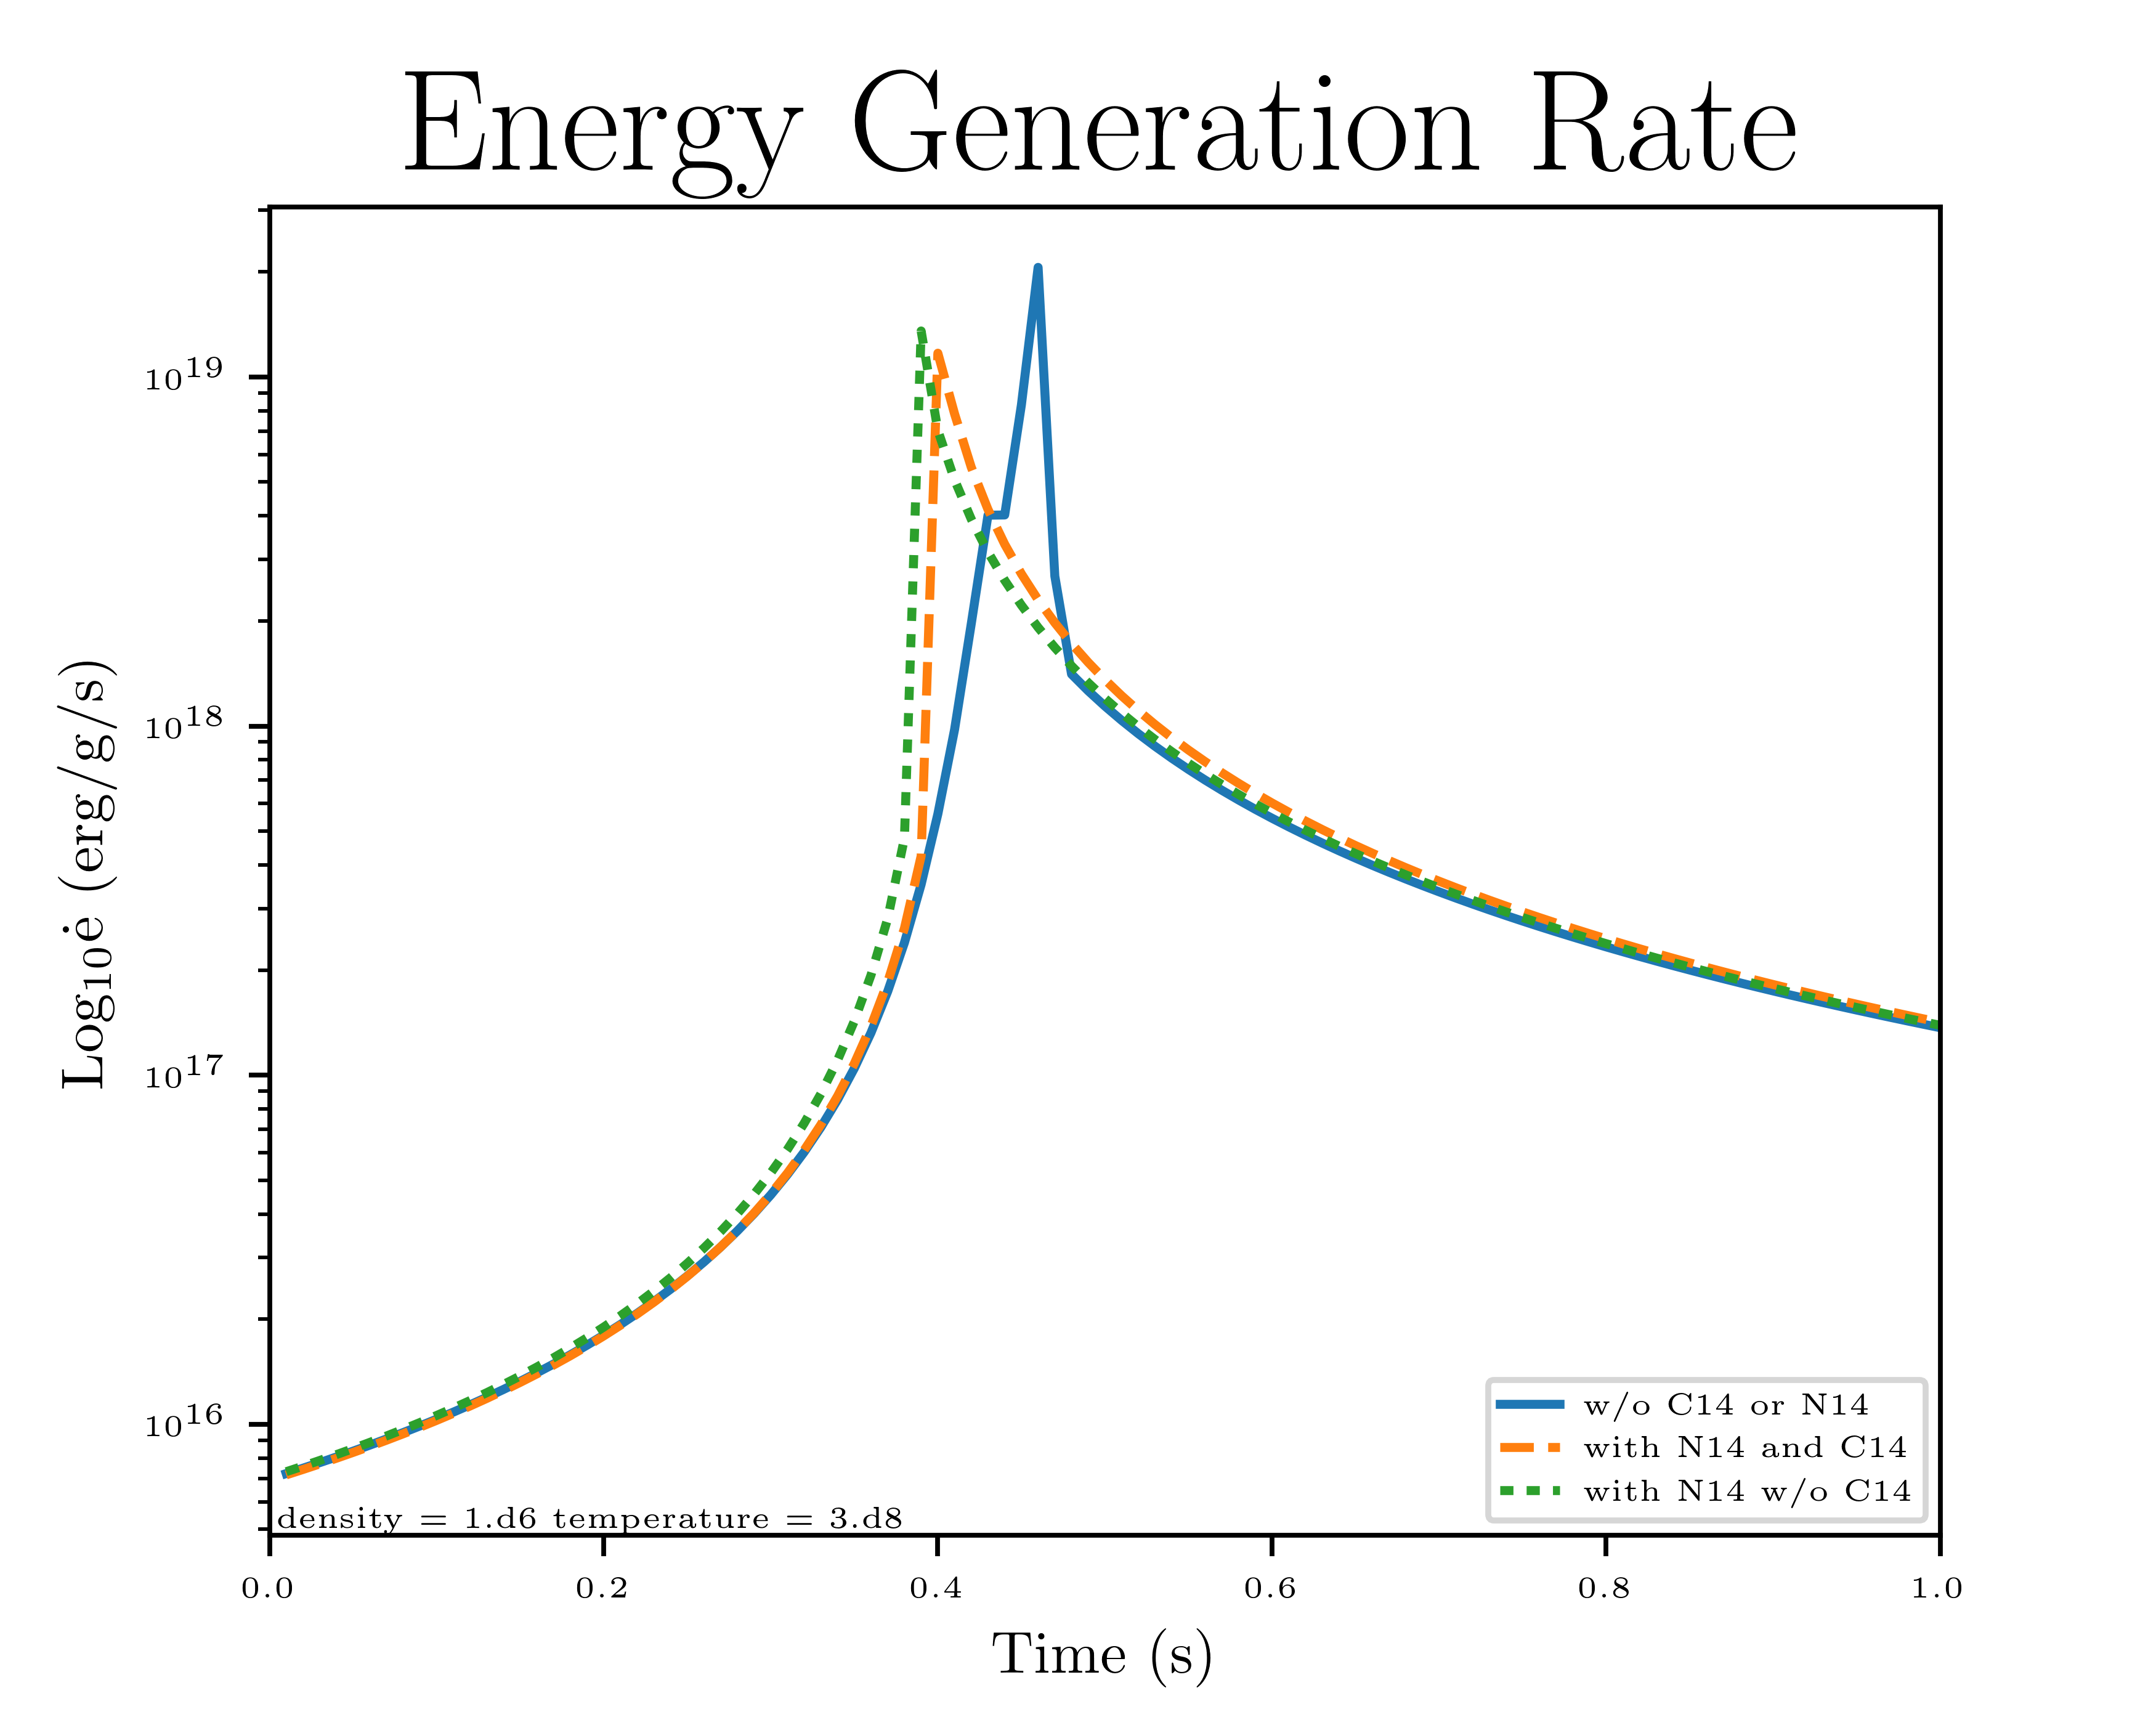
\includegraphics[width=5in]{images/subch_nC14nN14_edot_tol-10.png}
        \caption{}
        \label{fig:energygeneration}
      \end{figure} 
  
  \subsection{Castro}
  
    The Castro code will be used to first test the {\tt subch} network in one dimension to see if an increase in temperature will ignite a flame and push it across a layer of helium. If so, then the Castro code will be used to simulate the star in two dimensions. This can then be compared to simulations of stars using other networks and the results can be compared. 
    
    \subsection{1-Dimensional Simulations}
    
      Using the Castro science problem called "Detonation", a simulation of a flame propagating from left to right was initialized with the {\tt subch} network. As shown in Figure~\ref{fig:detonation}, when the left side of the helium layer is heated to 2 billion Kelvin, the energy released from nuclear reactions powers the flame wave to the right side of the screen and off of the page. 
      
      \begin{figure}
        \centering
        \includegraphics[width=0.5in]{}
        \caption{}
        \label{fig:detonation}
      \end{figure}
      
      Now, knowing that a mild temperature perturbation can ignite a helium layer, this simulation can be taken to two dimensions, which is a big step. These one dimensional simulations take a couple minutes to run on an average computer but the two dimensional simulations will take much longer. 
    
    \subsection{2-Dimensional Simulations}
  
      The two dimensional simulations are completed by wrapping a \ce{^{12}C} and \ce{^{16}O} WD core in a thick layer of \ce{^4He} then taking a half moon shaped slice of the WD and simulating the two dimensional burning in this slice. The burning is initiated by a hot temperature perturbation at the very top of the star on the star. Using the {\tt subch} network to simulate this, the images in Figure~\ref{fig:subchsims} resulted. 
      
      %Talk about the size and magnitude of the perturbation
      
      \begin{figure}
        \centering
        \includegraphics[width=5in]{}
        \caption{}
        \label{fig:subchsims}
      \end{figure}
      
      %Compare it to the aprox13 runs and talk about it.
  
\section{Conclusion}
  
  Previous simulations of Type Ia SNe %explain....
  Shen \& Bildsten's paper brought light to this issue, motivating the investigation narrated in this report. After checking the accuracy of codes simulations using a network of nuclear reaction rates based off of the Shen \& Bildsten paper were used in a one zone simulation, moving to a one dimensional simulation, and culminating in an insightful two dimensional simulation. It was proven that % fill this in when results exist. 
  
  The next steps moving forward will be to perform this in a three dimensional simulation. Using these results we can motivate fellow scientists to use their codes to retrieve the information about brightness curves and spectra so that observational astronomer can use them for calculating astronomical distance. Through the generation of better simulations, the scientific community gains better results and can produce excellent science. 
  
\end{document}  